% Ella-Lovise  is writing

\subsection*{Problem 2.4}
\addcontentsline{toc}{subsection}{Problem 2.4}

\subsubsection*{Calculate sideslip angle}
\addcontentsline{toc}{subsubsection}{Calculate sideslip angle}

The sideslip angle is as the angle from $x_b$ axis of {b} to the velocity vector of the vehicle, with positive rotation about the $z_b$ axis of {b} as given by the right-hand screw convetion. The formmula for sideslip is therfore:
\begin{equation}
    \boldsymbol{\beta}_r = \arcsin( v^b_r/U^b_r)
    \label{eq:beta_r}
\end{equation}
defined by the relative velocity $v_r$ and relative speed $U_r$. The relative velocity is defined as \eqref{eq:v_r}. To find the relative velocity it is necessary to rotate either the velocity of the vechicle or current. The relative velocity of the vehicle in body-reference frame is:

\begin{equation}
    \boldsymbol{v}^b_r = \boldsymbol{v}^b_{b/c} - \boldsymbol{v}^{b}_{c/n} =  \boldsymbol{v}^b_{b/c} - \mathbf{R}^b_n \boldsymbol{v}^{n}_{c/n} 
    \label{eq:v_b_r}
\end{equation}

The crab angle for the vehicle moving in the straight line was found by first calculating the realtive velocity, using equation \eqref{eq:v_b_r}, with  the velocity \todo{check to rephrase, of on seems a bit strange}of  on a straight line  $\mathbf{v}_b^b = [1.5, 0, 0]$, found in assignemnt 2.1, and   the current velocity was calculated in assignment 2.3, using equation \eqref{eq:v_n_c}. \todo{Should i say something about the approximation}. The crab angle was calculated using equation \eqref{eq:beta_r}, giving sideslip angle of $-9.6357 ^\circ$. \todo{check if Alexandra agree} This means the vehicle is moving upwards relative to current, relative to body-frame. This makes sense since the vehicle and the current are moving in same directions, the sideslip angle is negative. \todo{ CONFUSED, ASK ALEXANDRA!}

\subsubsection{Simulation of translational motion of the vehicle on the circle}

The simulation of the translational motion was done by simulation in \texttt{MATLAB}. The initial conditions were : \todo{SET INN INITIAL CONDITIONS }. To simulate the translational motion without current, the velocity of the vehicle was calculated first:
\begin{equation}
    \mathbf{v}^n_{b/n} = \mathbf{R}^n_b \mathbf{v}^b_{b/c} =\mathbf{R}^n_b \mathbf{v}^b_{b/n} = \mathbf{R}^n_b [U*cos(\omega t), U*sin(\omega t), 0]^\top
    \label{eq:v_n_b_c}
\end{equation}

Since there is no current, $\mathbf{v}^b_{b/c} = \mathbf{v}^b_{b/n}$.

The position of the vechicle was found by using Euler integration,meaning the position in needed for vehicle $\mathbf{p}(i+1)^n_b = \mathbf{p}(i)^n_b + \mathbf{v}(i)^n_b*h $, with $h = 0.1$, which is the simulation step.
 
The  simulation of the translational motion with current, was choosen to be relative to ned referance frame with the position relative to the ocean surface, and not relative to the current. \todo{Agree Alexandra? Jeg forstår ikke helt hva setningen sier..?}. The first step was to calculate the velocity of the vehicle $\mathbf{v}^n_{b/c}$, as done in \eqref{eq:v_n_b_c}. Furthermore the velocity of the current relative to ned, expressed in ned $\mathbf{v}^n_{c/n}$ was calculated, from equation \eqref{eq:v_n_c}. The expression for the velocity of the vehicle relative to ned reference frame and relative to the ocean surface (meaning vehicle is moving with current) is:

\begin{equation}
    \mathbf{v}^n_{b/n} = \mathbf{v}^n_{b/c} + \mathbf{v}^n_{c/n}
\end{equation}

The expression for the position of the vechicle relative to ned reference frame and relative to the ocean-surface is found by euler integration, meaning $\mathbf{p}(i+1)^n_b = \mathbf{p}(i)^n_b + \mathbf{v}(i)^n_b*h $, with $h = 0.1$. The method used is the same as for the simulation without current.

The relative velocity  in ned reference frame is by definition (referance \cite{Fossen2011} \todo{find reference}) of the vehicle is given as:

\begin{equation}
    \mathbf{v}^n_{r} = \mathbf{v}^n_{b/c} - \mathbf{v}^n_{c/n}
    \label{eq:v_n_r}
\end{equation}.

The crab angle, course angle and slip-angle was calculated using ??,?? and \eqref{eq:beta_r}, respectively. Because the arcsin command in \texttt{MATLAB},\texttt{asin} only provides angles between $\frac{\pi}{2}$ and $\frac{\pi}{2}$,the crab angle and sideslip angle was approximated using $atan2(u,v)$, approximating $w= 0$.

The plots after the simulation are:

\begin{figure}[!ht]
	\centering
	\begin{subfigure}[b]{0.45\textwidth}
		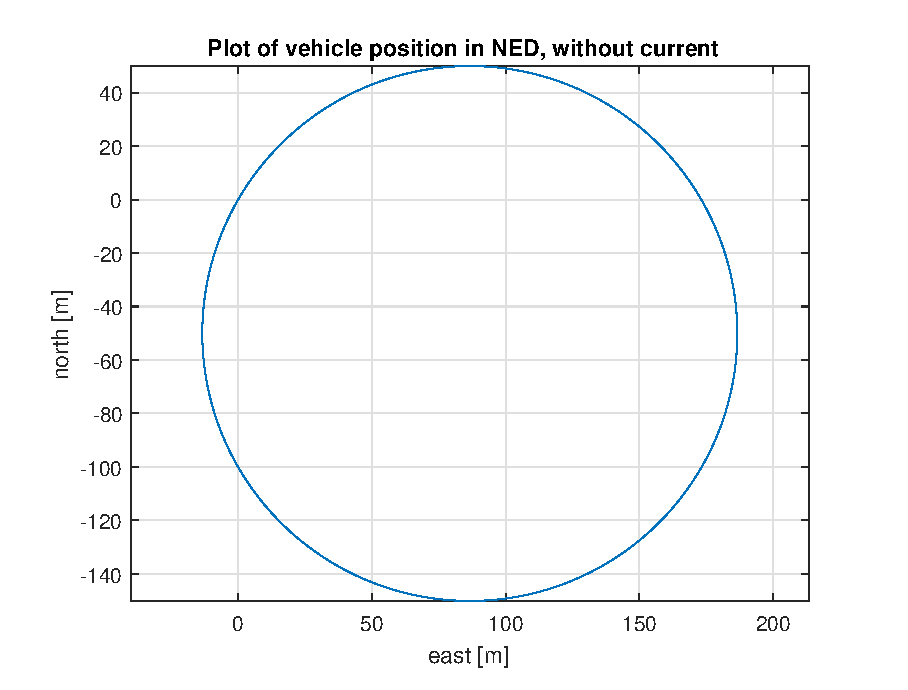
\includegraphics[width=\textwidth]{figures/4_pos.eps}
		\caption{Without current}
		%\label{fig:4_pos}
	\end{subfigure}
	~ %add desired spacing between images, e. g. ~, \quad, \qquad, \hfill etc. 
	%(or a blank line to force the subfigure onto a new line)
	\begin{subfigure}[b]{0.45\textwidth}
		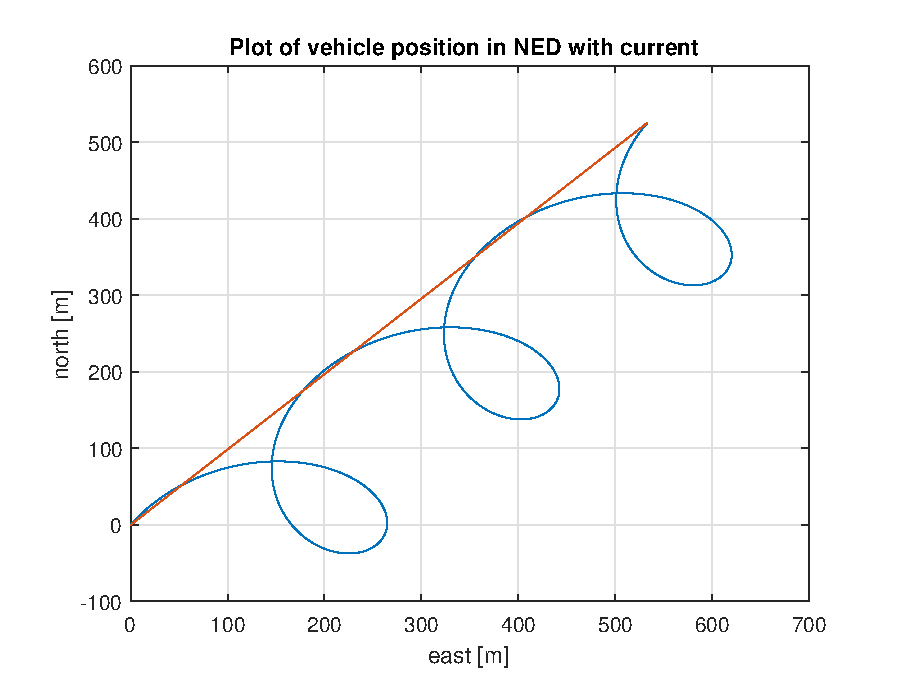
\includegraphics[width=\textwidth]{figures/4_pos_current}
		\caption{With current}
		%\label{fig:4_pos_current}
	\end{subfigure}
	\label{fig:4_pos}
	\caption{The position of the vehicle relative to ocean in reference frame ned}
\end{figure}

\begin{figure}[!ht]
	\centering
	\begin{subfigure}[b]{0.45\textwidth}
		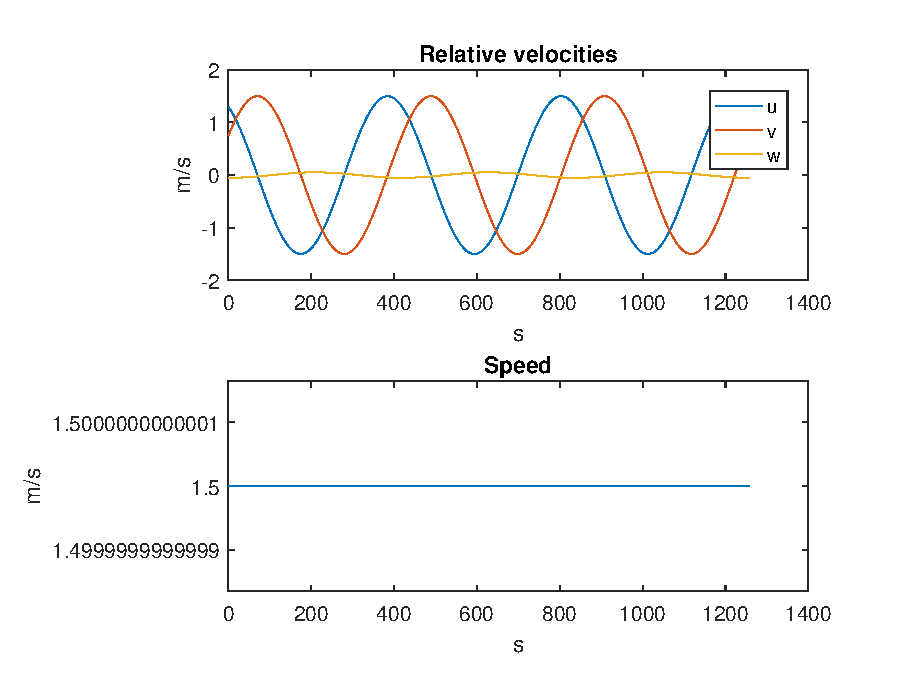
\includegraphics[width=\textwidth]{figures/4_vel}
		\caption{Without current}
		%\label{fig:4_vel}
	\end{subfigure}
	~ %add desired spacing between images, e. g. ~, \quad, \qquad, \hfill etc. 
	%(or a blank line to force the subfigure onto a new line)
	\begin{subfigure}[b]{0.45\textwidth}
		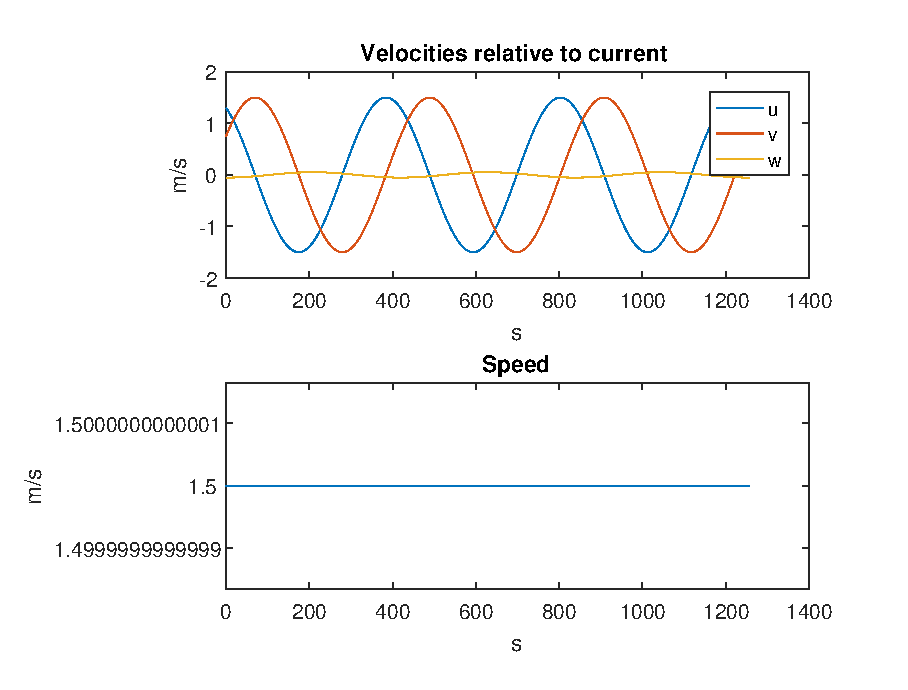
\includegraphics[width=\textwidth]{figures/4_vel_current}
		\caption{With current}
		%\label{fig:4_vel_current}
	\end{subfigure}
	\caption{The relative velocity and speed of the vehicle ,defined equation \eqref{eq:v_n_r}  in reference frame ned}
	\label{fig:4_vel}
\end{figure}

\begin{figure}[!ht]
	\centering
	\begin{subfigure}[b]{0.45\textwidth}
		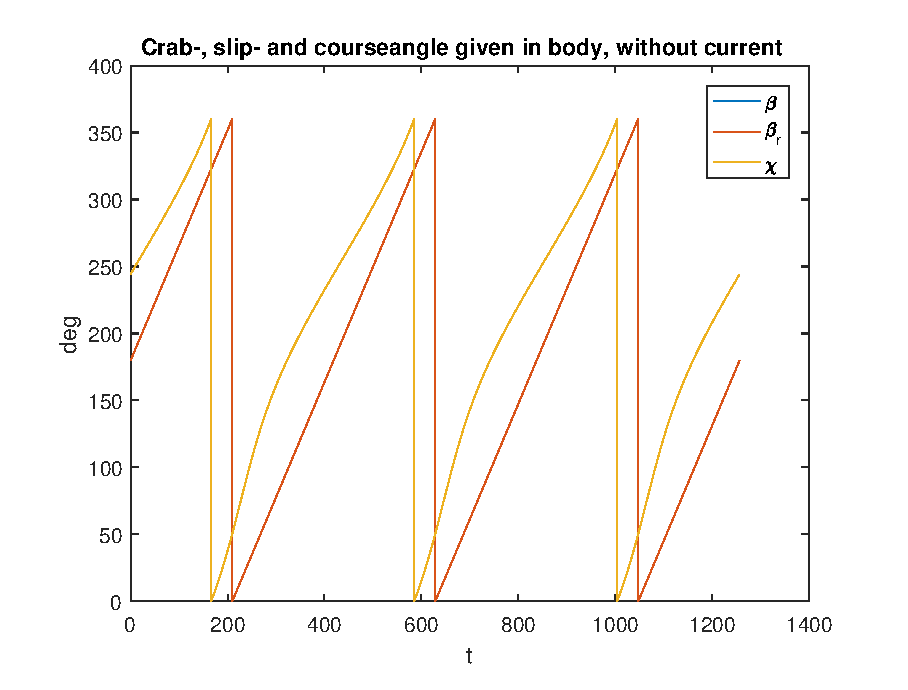
\includegraphics[width=\textwidth]{figures/4_crab_slip_course}
		\caption{Without current}
		%\label{fig:4_vel}
	\end{subfigure}
	~ %add desired spacing between images, e. g. ~, \quad, \qquad, \hfill etc. 
	%(or a blank line to force the subfigure onto a new line)
	\begin{subfigure}[b]{0.45\textwidth}
		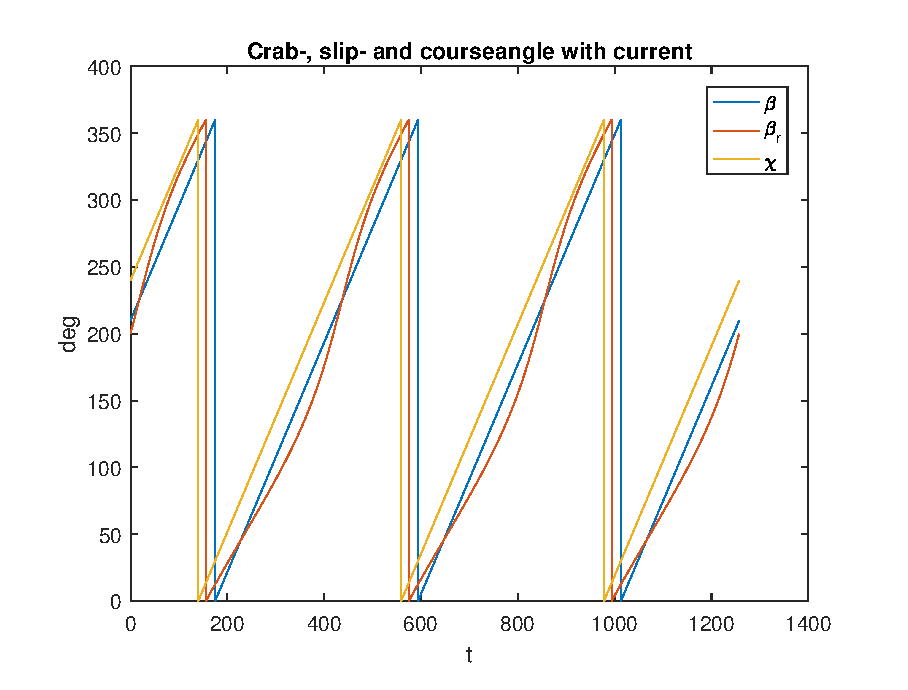
\includegraphics[width=\textwidth]{figures/4_crab_slip_course_current}
		\caption{With current}
		%\label{fig:4_vel_current}
	\end{subfigure}
	\label{fig:4_crab}
	\caption{The crab-, course and sidslipangle  in reference frame ned}
\end{figure}

In figure \figref{fig:4_pos} the position of the vehicle realtive to the ocean is plotted using reference frame ned. Without current the vehicle makes a perfect circle with radius 100 m., as required and expected. With current the vehicle tries to make a perfect circle, but the current carries the vehicle upwards, making the path to the vehicle relative to  the ocean looking like a spiral. This is as expected, since the vehicle has velocity to drive in a circle (relative to the current), but the current carries the vehicle upstream, which makes the path of the vehicle relative to the ocean surface look as a spiral.

The relative speed, defined as $v_r = v - v_c$, for the vehicle in NED reference frame is shown in figure \figref{fig:4_vel}. The relative speed of the vehicle without current is constant, since the current is zero, and $v^b_{b/c}=v^b_{b/n}$ and this is consistent of $[U \sin(\omega *t), U \cos(\omega*t),0]^\top$ the non rm value is $U = 1.5 m/s$. Since there is also current then, the relative speed of the vehicle in reference frame NED is affected by the current. Because the relative velocity is $v_r = v - v_c$, and $\mathbf{v}_c != \mathbf{0}$, the speed is not constant, but varies sinusoidally. \todo{any explanation why sinusoidal other than this ? Should i explain it more ?}

The plots of crab angle, slip angle and course angle goes from $0-360^\circ$. This is reasonable since the boat is driving in a circle with the "snout" \todo{check expression, snute på engelsk} in the same direction. In the plot without current $\mathbf{v}^b_{b/c} = \mathbf{v}^b_{b/n} $, this means $\beta_r = \beta$, and is the same result as from the plot. In the plot with current the course angle and beta are the same as in plot without current, while the slip angle varies because of the current velocity not being zero. Since there is current both the relationship between $u^b_r$ and $v^b_r$ varies periodically, meaning the side slip angle varies periodically. The reason for the current and course angle behaving this way is the same, since they are not dependent on the current velocity. \todo{Check with Alexandra if the crab angle should be v\_b\_b\_c or v\_b\_b\_n in the equation} .

\subsection*{Problem 2.5}

The vehicle's turning rate is now assumed to be modeled by the Nomoto model and are:
\begin{equation}
	\frac{r}{\delta} (s) = \frac{K}{Ts+1}
\end{equation}

with $\delta$ equal the rudder angle, $K =0.1 s^{-1}$ and $T = 50s$.

The pitch and rollmotions are given as
\begin{equation}
\begin{aligned}
	&\dot{p} + 2\zeta_p\omega_p p + \omega_p^2 \phi = 0\\
	&\dot{q} + 2\zeta_q\omega_q q + \omega_q^2 \theta = 0
	\label{eq:p_q_dot}
\end{aligned}
\end{equation}
with damping factors and natural  frequencies as $\zeta_p = 0.1 $, $\zeta_q = 0.2 $, $\omega_p = 0.1 $ and $\omega_q = 0.05 $. 

\subsubsection*{Calculations of steady state}

The steady state angular velocities $p_s$, $q_s$ and $r_s$ during turning for a constant rudder angle $\delta$ may be found by setting $\dot{p}= \dot{q} = \dot{r} = 0$. The equation for $\dot{r}$ may be found by inverse Laplace using the Nomoto equation. In \cite{Fossen2011} the time representation of the first order Nomotos model, equation (7.52) in \cite{Fossen2011} is estimated as 

\begin{equation}
    T \ddot{\psi} + \dot{\psi} = K \delta
    \label{eq:nomo_first_order_time}
\end{equation}

In this problem $\theta = 2.0 ^\circ$ and $\phi = 0.0 ^\circ$, giving $\dot{\psi}$ as approximately $r$. Using \eqref{eq:nomo_first_order_time} the  first order Nomo-model time representation as:

\begin{equation}
    T \dot{r} + r = K \delta
    \label{eq:r_time}
\end{equation}

Using \eqref{eq:r_time} and \eqref{eq:p_q_dot} and setting $\dot{p} =\dot{q} = \dot{r}$ gives the following expression for the seaty state of the linear velocities $\dot{\omega}^b_{b/n}$:

\begin{equation}
\begin{aligned}
	& p_s = \frac{\omega_p^2 \phi}{ 2\zeta_p\omega_p} \\
	& q_s = \frac{\omega_q^2 \theta}{2\zeta_q\omega_q} \\
	& r_s = K \delta
	\label{eq:p_q_dot}
\end{aligned}
\end{equation}

Using $\theta = 2.0$, $\phi = 0$ gives the steady-state velocities $p_s = 0$, $q_s = 0.1 ^\circ$, $r_s = 0.1 \delta$. This means that in steady state, there is approximately no angular velocities around $x_b$ and $y_b$, while around $z_b$ there is a constant angular velocity, meaning the vehicle will turn in a circle about $z_b$ as long as there is rudder. \todo{Alexandra, anything to add ?}

\subsection*{Problem 2.6}


References can be placed in the bibliography.bib and referred to as \cite{Fossen2011} and \cite{Fjellstad1994857}.


% files added by teacher

Answer Problem 2.4 here. Figures can be inserted as:
\begin{figure}[ht]
	\centering
	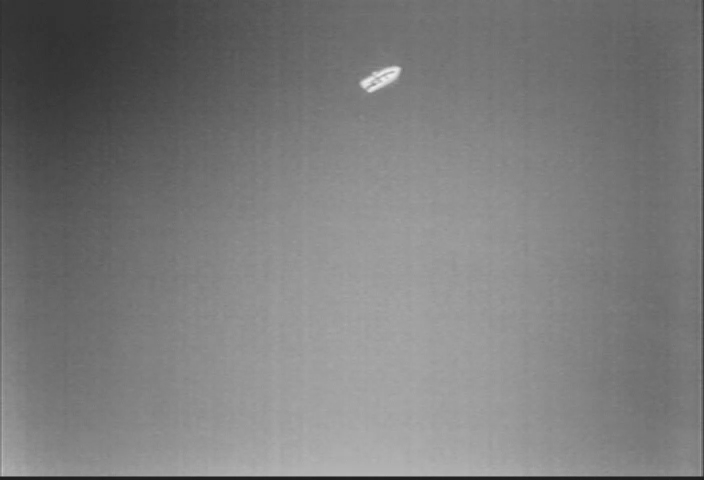
\includegraphics[width=0.7\textwidth]{assignment_1/rapport/figures/fig1} 
	\caption{Figure of something useful.}
	\label{fig:fig1}
\end{figure}

You can now refer to this figure as \figref{fig:fig1}. You can also insert figures side-by-side:
